\subsection{Principle Component Analysis}

In this section, we discuss the performance of our SVD-based algorithms in terms 
of their speed and correctness.

\subsubsection{Singular Value Decomposition}

\begin{center}
    \textbf{Correctness}
\end{center}

In numerical methods such as SVD, the accumulation of floating point error prevents us from measuring exact correctness.
Instead, we define some small $\varepsilon$, and consider two matrices $A \approx_\varepsilon B$ to be ``basically equal'' if 
for all $i, j$, $|a_{ij} - b_{ij}| < \varepsilon$. When testing on large matrices, we chose $\varepsilon = 1 \times 10^{-5}$
to be our goal, though in practice on smaller matrices ($m, n \leq 50$) we attain correctness up to $\varepsilon = 1 \times 10^{-9}$.

To test correctness of our SVD implementation, we start with a randomly generated matrix $A \in \R^{m \times n}$
where each entry is sampled from the normal distribution $\mathcal N(0, 1)$, and compute its SVD into $U$, $V$, 
and $\Sigma$. We then check that $U$ and $V$ are orthogonal by testing $U^\top U \approx_\varepsilon I_m$ 
and $V^\top V \approx_\varepsilon I_n$. We then check that $A \approx_\varepsilon U \Sigma V^\top$. 

Sometimes, our SVD implemention does not converge on a particular matrix, and so we abort the execution. The main loop 
of the Golub-Kahan algorithm should in theory take $\mathcal O(n)$ steps, so we introduced a check that if the main loop
runs more than $30n$ times, we declare the instance a failure, and return empty $0 \times 0$ matrices.

With $m$ and $n$ sampled randomly in the range $2$ through $20$, we ran the above testing proceedure 10,000 times and 
found no correctness failures, though we observe a divergence rate of about $2.49\%$. That is, on small matrices, our 
algorithm failed to converge on 249 out of the 10,000 random matrices.

The issue of convergence seems to become better with larger matrices. When we sample $m$ and $n$ randomly from the range 
$2$ through $200$, we found that out of 300 trials, only 1 instance failed to converge, a rate of $.33\%$.

For matrices with $200 \leq m, n \leq 300$, we found no matrices with failed to converge out of 30 trials.

\begin{center}
    \textbf{Runtime Performance}
\end{center}

Our SVD implementation is absurdly slow. It became impractical to test at a large scale for matrices with more than 
$500 \times 500 = 250,000$ entries. This is unfortunate, as most real-world applications would require much larger 
matrices. When we first tried image compression, we used a 4K image taken by an iPhone, and running SVD on 
each color channel took so long that even when let to run for 12 hours overnight, it didn't terminate. It is hard to 
know if this is because it genuinely just took so long, or if it fell into the small fraction of cases that caused 
divergence. Because of the decaying rate of divergence for larger dimensions, we believe it is the former. We also 
tried running SVD on matrices of comparable size (with $m$ and $n$ in the low thousands) and were unable to get 
it to terminate after several hours.

This is almost certainly due to the fact that at this stage of development we did \emph{not} fully optimize our 
Golub-Kahan implementation. The first step, which relies on bi-diagonalizing the matrix, uses a sequence of Householder 
reflections, which if implemented efficiently can take linear time as they only affect two rows of a matrix. Further 
optimization would include only applying the reflection to a sub-matrix of $A$, and not the entire matrix. Instead, 
we applied the householder reflection matrix to the entire matrix $A$, taking $\mathcal{O}(n^3)$ time for each step.
This easily balloons the runtime, since this is done inside an inner loop. At first, we tried implementing 
the fully optimized Golub-Kahan algorithm, but were unable to get it to work correctly. So, we focused on just 
trying to get a \emph{correct} implementation instead of premature optimization. The natural next steps after this 
project would be to get this running faster!

\subsubsection{Image Compression}

As discussed above, we were unable to run our image compression on large images, so we started with low-resolution 
images. We ran our image compression algorithm on two images, one of some sheep,\ftntmk{}\footnotetext{The 
sheep are in the teaching barn by the Vet School. I highly recommend that you go visit and pet them! It's 
free and you can just walk right up to them!}, and one 
of a cat. 

When a matrix $A$ is decomposed into $U, \Sigma, V$, and all but the first $k$ singular values are ditched, we are 
left with three matrices of sizes $m \times k$, $k$ and $n \times k$ (we need only store the diagonal of $\Sigma$).
So, the number of floating point values we must store as a fraction of the amount we would need to fully represent 
$A$ is what we call the ``compression ratio,'' computed as 
\[
    r = \frac{r + rm + rn}{mn}
\]
For small matrices and large values of $r$, this doesn't save much. However, this scales incredibly well for large matrices, 
as we can pick modestly small values of $r$ and end up with impressive compression ratios while still being able to recognize 
the original image. A small caveat here is that typically a single pixel's channel for one color only uses one byte to 
represent it, whereas we are using 64-bit floating points, so one could argue that we need to include a factor of 8 
in our compression ratio. However, our compression would work just as well if each color channel was represented 
as a floating point value between 0 and 1 (since this is what we convert the image to anyway when we begin 
compression), so we think it is fair to compare the sizes when thinking of the original channel as being a 
decimal between 0 and 1 as opposed to an integer between 0 and 255.

\begin{center}
    \textbf{Sheep}
\end{center}

We used a $240 \times 320$ pixel image of some sheep laying in a barn, and truncated the singular values
up to the first $k \in \{100, 50, 10\}$. Running SVD to decompose the image took \textbf{1m 15s}.

\begin{figure}[H]
  \centering
  \begin{minipage}[b]{0.4\textwidth}
    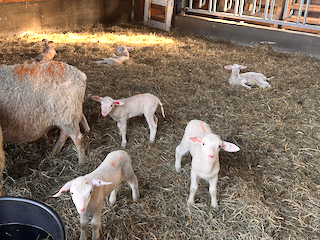
\includegraphics[width=\textwidth]{images/sheep.png}
    \caption{Original}
  \end{minipage}
  \hfill
  \begin{minipage}[b]{0.4\textwidth}
    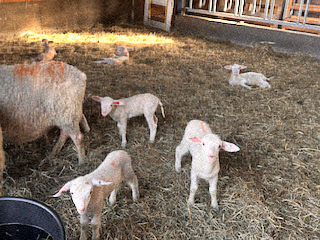
\includegraphics[width=\textwidth]{images/compressed_sheep_100.png}
    \caption{$k = 100$, $73.0\%$ compression}
  \end{minipage}
\end{figure}

\begin{figure}[H]
  \centering
  \begin{minipage}[b]{0.4\textwidth}
    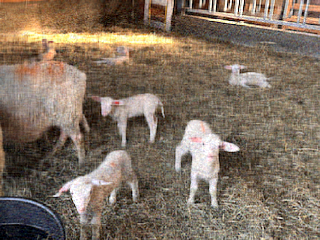
\includegraphics[width=\textwidth]{images/compressed_sheep_50.png}
    \caption{$k = 50$, $36.5\%$ compression}
  \end{minipage}
  \hfill
  \begin{minipage}[b]{0.4\textwidth}
    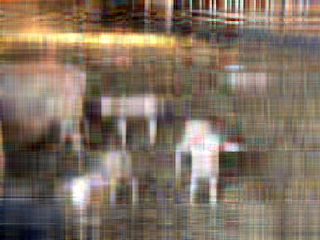
\includegraphics[width=\textwidth]{images/compressed_sheep_10.png}
    \caption{$k = 10$, $7.3\%$ compression}
  \end{minipage}
\end{figure}

\begin{center}
    \textbf{Panini (the cat)}
\end{center}

On a $640 \times 480$ image of Panini, SVD took \textbf{20m 50s} to finish. Here are the results 
using the first $k \in \{150, 50, 7\}$ singular values.

\begin{figure}[H]
  \centering
  \begin{minipage}[b]{0.4\textwidth}
    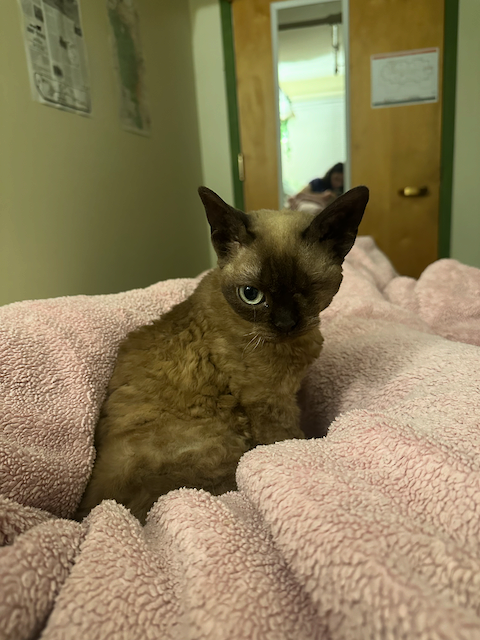
\includegraphics[width=\textwidth]{images/cat.png}
    \caption{Original}
  \end{minipage}
  \hfill
  \begin{minipage}[b]{0.4\textwidth}
    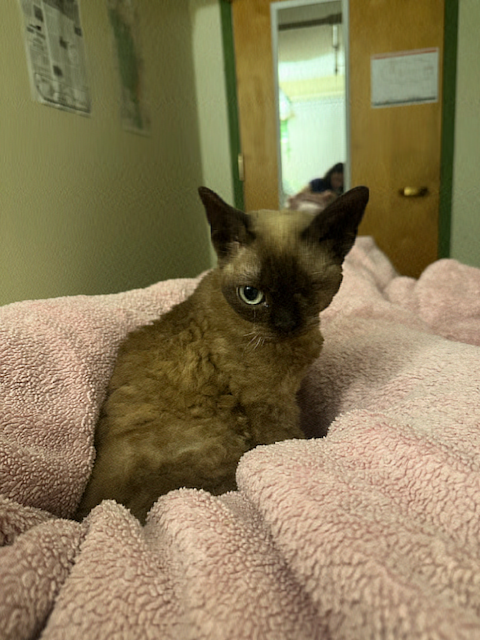
\includegraphics[width=\textwidth]{images/compressed_cat_150.png}
    \caption{$k = 150$, $54.7\%$ compression}
  \end{minipage}
\end{figure}

\begin{figure}[H]
  \centering
  \begin{minipage}[b]{0.4\textwidth}
    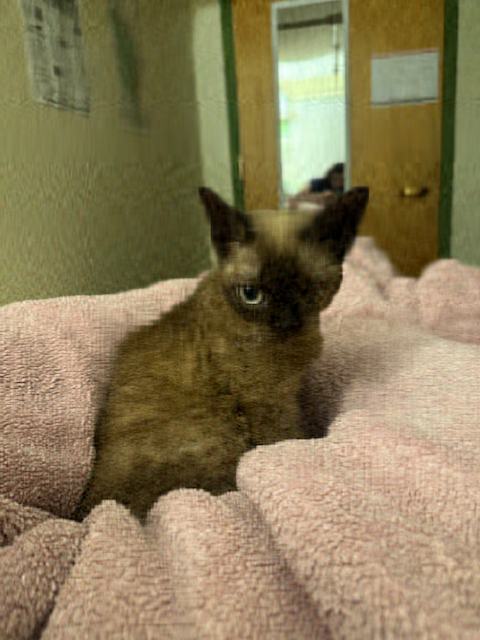
\includegraphics[width=\textwidth]{images/compressed_cat_50.png}
    \caption{$k = 50$, $18.2\%$ compression}
  \end{minipage}
  \hfill
  \begin{minipage}[b]{0.4\textwidth}
    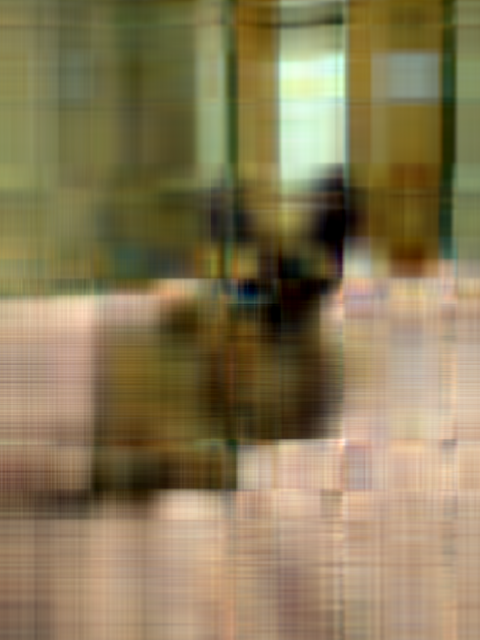
\includegraphics[width=\textwidth]{images/compressed_cat_7.png}
    \caption{$k = 7$, $2.6\%$ compression}
  \end{minipage}
\end{figure}

\subsubsection{Planes of Best Fit}